\documentclass{beamer}
\usepackage[utf8]{inputenc}
\usepackage{listings}
\usepackage{booktabs}
\usepackage{amssymb}
\usepackage{amsmath}
\usepackage{bm}
\usepackage{enumitem}
\usepackage{hyperref}
\usepackage[export]{adjustbox}
\usepackage{svg}

\usetheme{Madrid}
\definecolor{mlpblue}{rgb}{0.1, 0.14, 0.24}

\useoutertheme{infolines} % Alternatively: miniframes, infolines, split
\useinnertheme{circles}
\usecolortheme[named=mlpblue]{structure}

\lstset{basicstyle=\footnotesize\ttfamily,breaklines=true}

%------------------------------------------------------------
%This block of code defines the information to appear in the
%Title page
\title[DPO]{Direct Preference Optimization:}

\subtitle{Your Language Model Is Secretly a Reward Model\thanks{Rafailov, Sharma, Mitchell, et. al}}

\author[Machine Learning @ Purdue] % optional
{J.~Setpal} 

\date{\today}

\titlegraphic{
\includegraphics[width=7cm]{../shared/logo-long.pdf}}

%End of title page configuration block
%------------------------------------------------------------

%The next block of commands puts the table of contents at the 
%beginning of each section and highlights the current section:

\AtBeginSection[]
{
  \begin{frame}
    \frametitle{Outline}
    \tableofcontents[currentsection]
  \end{frame}
}
% ------------------------------------------------------------


\begin{document}

\frame{\titlepage}


%---------------------------------------------------------
% This block of code is for the table of contents after
% the title page
\begin{frame}
\frametitle{Outline}
\tableofcontents
\end{frame}
%---------------------------------------------------------

\section{Background, Intuition, Motivations}
\bgroup
\let\oldfootnoterule\footnoterule
\def\footnoterule{\only<3->\oldfootnoterule}
\begin{frame}{Task Formulation}
	Consider the sample conversation: \\
	\textbf{Human:} What is your favourite pet? \\
	\textbf{LLM:} I like \_\_\_\_\_\_\_ \newline \\

	\textbf{Q:} What's the \textit{correct} answer? \pause Dog? Cat? Human? Something else? \pause \\
	\textbf{A:} Depends\footnote<3->{But still, definitely not human.} on our \textit{preferences}. \pause \newline \\

	\underline{Preference Modelling} involves embedding subjective biases within LLMs. \pause \newline \\

	Following are two popular objective models DPO solves for:
	\begin{enumerate}[label=\alph*.]
		\item \textbf{Bradley-Terry:} Binary result ranking -- $y_1 \succ y_2$
		\item \textbf{Plackett-Luce:} Multi-result ranking -- $y_1 \succ y_2 \succ y_3 \succ \ldots \succ y_n$ 
	\end{enumerate}
\end{frame}
\egroup

\begin{frame}{RLHF Synopsis (1/2)}
	We'll review the RLHF pipeline per Zeiger et al. It has 3-primary phases:
	\begin{enumerate}[label=\arabic*.]
		\item \textbf{Supervised Fine-Tuning (SFT)}: A pre-trained LLM ($\pi_{PT}$) is fine-tuned on \underline{high-quality}, domain-specific datasets to obtain $\pi_{SFT}$. \pause
		\item \textbf{Reward Modelling:} Next, we obtain a reward model $r_\phi(x,y)$ that models user preferences. \pause We start by sampling from $\pi_{SFT}$:
			\begin{gather}
				\mathcal{D} := \{(x_j, y_1, y_2)\}^{N,K}_{i=1,j=1} \sim \pi_{SFT}(y|x), \{x_i\}^K_{i=1} \\
				y_w \succ y_l | x \sim r^*(x,y)~\forall~(y_1, y_2) \in \mathcal{D}
			\end{gather}
			where $r^*(x,y)$ is the unknown optimal policy. \pause Per Bradley-Terry:
			\begin{gather}
				p^*(y_1 \succ y_2 | x) = \sigma_{softmax[y_1]}(r^*(x,y));~y \in \{y_1, y_2 \} \label{eq:3}
			\end{gather}
			is the preference distribution optimized over \underline{negative log-likelihood} on a parameterized model $r_\phi(x,y)$. \pause Some notes:
			\begin{enumerate}[label=\alph*.]
				\item Rewards are normalized over $x$ to motivate lower variance. \pause
				\item $r_\phi$ is $\pi_{SFT}$ with the final linear layer returning the scalar reward.
			\end{enumerate}
	\end{enumerate}
\end{frame}

\begin{frame}{RLHF Synopsis (2/2)}
	\begin{enumerate}
		\item[3.] \textbf{RL Fine-Tuning:} Finally, we use $r_\phi$ to fine-tune $\pi_{SFT}$, with the following objectives:
			\begin{enumerate}[label=\alph*.]
				\item $r_\phi$ should be maximized. \textbf{Assumption:} $r^* \approx r_\phi$. \pause
				\item We \textit{do not} want mode-collapse (random tokens that maximize reward). \pause \textbf{Solution:} \underline{KL Divergence}. \pause
			\end{enumerate}
			Mathematically, RLHF posits the following optimization problem:
			\begin{gather}
				\max_{\pi_\theta}\mathbb{E}_{x\sim\mathcal{D}, y \sim \pi_\theta(y|x)}(r_\phi(x,y)) -\beta \mathbb{D}_{KL}[\pi_\theta(y|x)~||~\pi_{SFT}(y|x)]
			\end{gather} \pause
			This is equivalent to the reward function:
			\begin{gather}
				r(x,y) = r_\phi(x,y) - \beta(\log \pi_\theta(y|x)) - \log(\pi_{SFT}(y|x))
			\end{gather}
			Which is maximized using \textbf{Proximal Policy Optimization}.
	\end{enumerate}
\end{frame}

\bgroup
\let\oldfootnoterule\footnoterule
\def\footnoterule{\only<6->\oldfootnoterule}
\begin{frame}{Why DPO?}
	The primary issue with using RLHF is \underline{language generation is discrete}. \pause \\

	As a consequence, the objective is \textbf{non-differentiable}. \pause \newline \\

	\underline{Actor-Critic Algorithms are unstable} because of the \textbf{normalization term}:
	\begin{gather}
		\hspace{-0.7em}
		\color{gray} \max_{\pi_\theta} \mathbb{E}_{\pi_\theta(y|x)} \left[r_\phi(x,y) {\color{black} -\beta \log\sum_y\pi_{SFT}(y|x)\text{exp}\left(\frac{r_\phi(x,y)}{\beta}\right)} - \beta \log \frac{\pi_\theta(y|x)}{\pi_{SFT}(y|x)} \right]
	\end{gather}
	High variance $\propto$ instability, and the normalization term is hard to optimize. \pause This can be learned or sampled by human-completion baselines. \pause \newline \\

	\vspace{-0.4em}
	DPO creates $r_\phi$ that enables optimal policy extraction \underline{in closed form}. \pause \newline \\

	\vspace{-0.4em}
	The optimization policy represents both: the language model and \textit{implicit} reward, that is optimized with log-loss.\footnote<6->{``Your Language Model Is Secretly a Reward Model''}
\end{frame}
\egroup

\section{Deriving \& Understanding DPO}
\begin{frame}{Objective}
	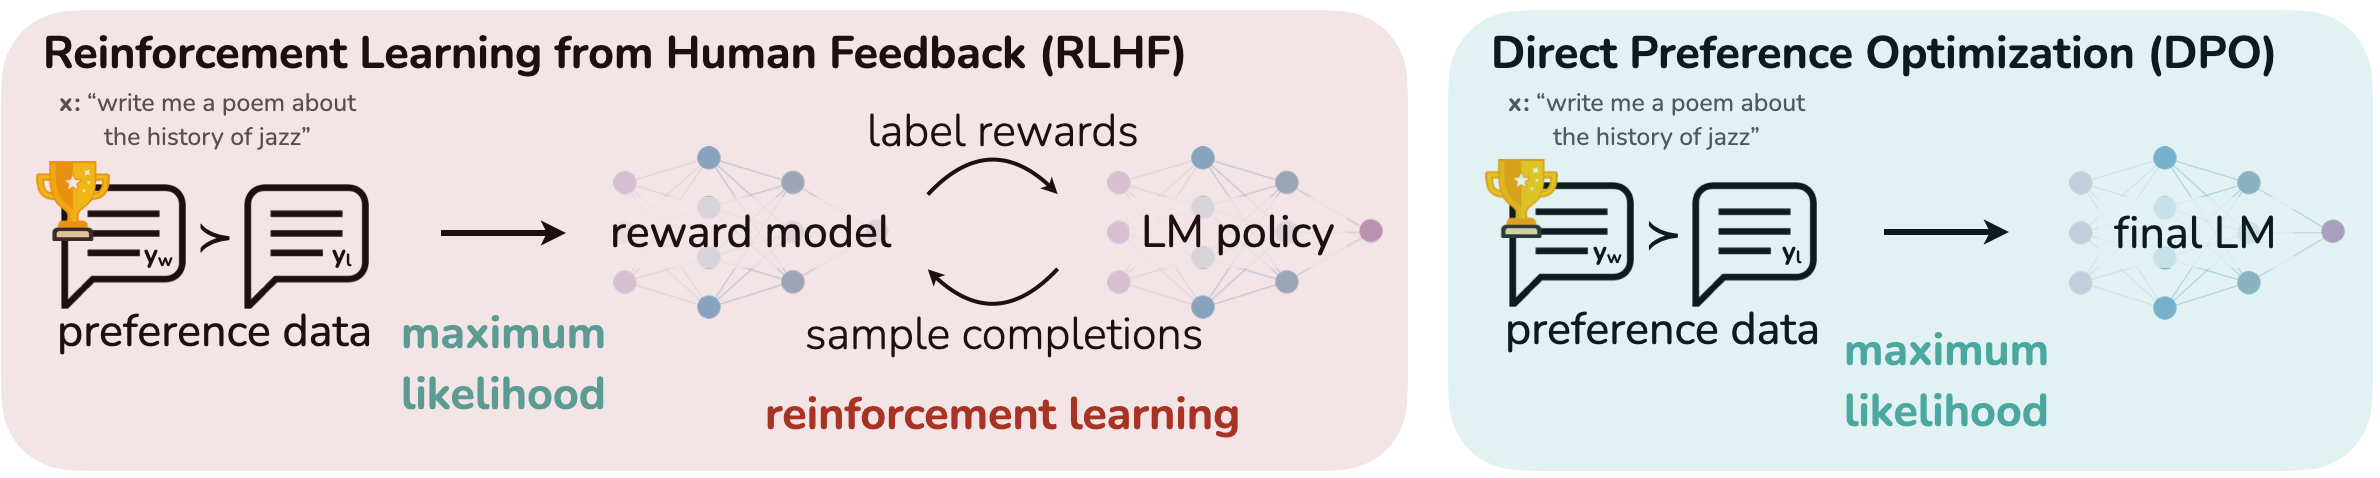
\includegraphics[width=\textwidth]{img/dpo-vs-rlhf.png} \pause \newline \\

	\underline{Objective:} Loss over \textit{reward} $\stackrel{Tr}{\rightarrow}$ Loss over \textbf{policy}. \pause \newline \\
	We must first identify $(\pi_{SFT},r) \stackrel{Tr}{\rightarrow} \pi^*$; $\pi^*$ is a \underline{valid probability distribution}. \pause \newline \\

	We use this to construct $\mathcal{L}_{DPO}$ which maximizes NLL over $\mathbb{D}_{KL}(\pi_\theta, \pi^*)$. \pause \newline \\

	If $\pi_{SFT}$ is not available, we obtain it by training $\pi_{PT}$ for the MLE:
	\begin{gather}
		\pi_{SFT} \stackrel{def}{=} \max_{\pi_{PT}} \mathbb{E}_{\{x, y_w\} \sim \mathcal{D}}(\log(\pi_{PT}(y_w|x)))
	\end{gather}
	which minimizes distribution shift.
\end{frame}

\begin{frame}{Finding $(\pi_{SFT},r) \stackrel{Tr}{\rightarrow} \pi^*$ (1/2)}
	We begin by restructuring the maximization objective from RLHF:
	\begin{align}
		&\max_{\pi_\theta}\mathbb{E}_{x\sim\mathcal{D}, y \sim \pi_\theta(y|x)}(r_\phi(x,y)) -\beta \mathbb{D}_{KL}[\pi_\theta(y|x)~||~\pi_{SFT}(y|x)] \tag{4} \\
		&= \min_{\pi_\theta}\mathbb{E}_{x \sim \mathcal{D}}\mathbb{E}_{y \sim \pi_{\theta}(y|x)} \left[ \log \frac{\pi_\theta(y|x)}{\frac{1}{Z(x)} \pi_{SFT}(y|x)\exp\left(\frac{1}{\beta}r(x,y)\right)} - \log Z(x) \right]
	\end{align}
	Where $Z(x)$ is a partition function (scalar that induces \underline{proportionality}). \pause \newline

	In English this time, here's what's happening:
	\begin{enumerate}[label=\arabic*.]
		\item The maximization objective is reward minus KL divergence. \pause
		\item $\max \stackrel{Tr}{\rightarrow} \min$ objective is divergence minus reward. \pause
		\item We can combine reward and the SFT model by plugging in a partition function.
	\end{enumerate}
\end{frame}

\begin{frame}{Finding $(\pi_{SFT},r) \stackrel{Tr}{\rightarrow} \pi^*$ (2/2)}
	From our new objective, we extract on optimal policy $\pi^*$:
	\begin{gather}
		\color{gray} \min_{\pi_\theta}\mathbb{E}_{x \sim \mathcal{D}}\mathbb{E}_{y \sim \pi_{\theta}(y|x)} \left[ \log \frac{\pi_\theta(y|x)}{\color{black} \frac{1}{Z(x)} \pi_{SFT}(y|x)\exp\left(\frac{1}{\beta}r(x,y)\right)} - \log Z(x) \right] \tag{8} \\
		\pi^*(y|x) = \frac{1}{Z(x)} \pi_{SFT}(y|x)\exp\left(\frac{1}{\beta}r(x,y)\right)
	\end{gather} \pause
	From here, we log both sides and solve for $r(x,y)$:
	\begin{gather}
		r(x,y) = \beta \left[\log \frac{\pi^*(y|x)}{\pi_{SFT}(y|x)} + \log(Z(x)) \right] \label{eq:10}
	\end{gather} \pause
	This is \textit{still} unsolvable, because it's hard to approximate $Z(x)$. However, we can fit this to the \textbf{Bradley-Terry Model}.
\end{frame}

\begin{frame}{Obtaining $\mathcal{L}_{DPO}$}
	Recall from RLHF definition, we have eq. \eqref{eq:3}:
	\begin{gather}
		p^*(y_1 \succ y_2 | x) = \sigma_{softmax[y_1]}(r^*(x,y));~y \in \{y_1, y_2 \} \tag{3}
	\end{gather}
	$\frac{d Z(x)}{dy} = 0$, so it does not play a role in optimization. \pause We get:
	\begin{gather}
		p^*(y_1 \succ y_2 | x) = \sigma_{softmax}\left( \beta \log \frac{\pi^*(y_1|x)}{\pi_{SFT}(y_1|x)} - \beta \log \frac{\pi^*(y_2|x)}{\pi_{SFT}(y_2|x)} \right)
	\end{gather}
	which is loss over a single sample. \pause \newline \\

	\textit{Finally}, we can maximize expectation over $p^*(y_1 \succ y_2 | x)$ with NLL:
	\begin{gather}
		\mathcal{L}_{DPO} = - \mathbb{E}_{(x,y_w,y_l) \sim \mathcal{D}} [ \log (p^*(y_1 \succ y_2 | x)) ] 
	\end{gather}
	over which we find our MLE.
\end{frame}

\section{Results}
\begin{frame}{Benchmark Scores}
	DPO's authors evaluated their approach on the following tasks:
	\begin{enumerate}[label=\arabic*.]
		\item \textbf{Controlled Sentiment Generation}
		\item \textbf{Text Summarization}
		\item \textbf{Single-Turn Dialogue}
	\end{enumerate}
	They used GPT-4 to perform `auto-evaluations' on the data, by asking GPT-4 to select a winner output through blind testing. \pause \newline \\

	\begin{columns}
		\begin{column}{0.33\textwidth}
			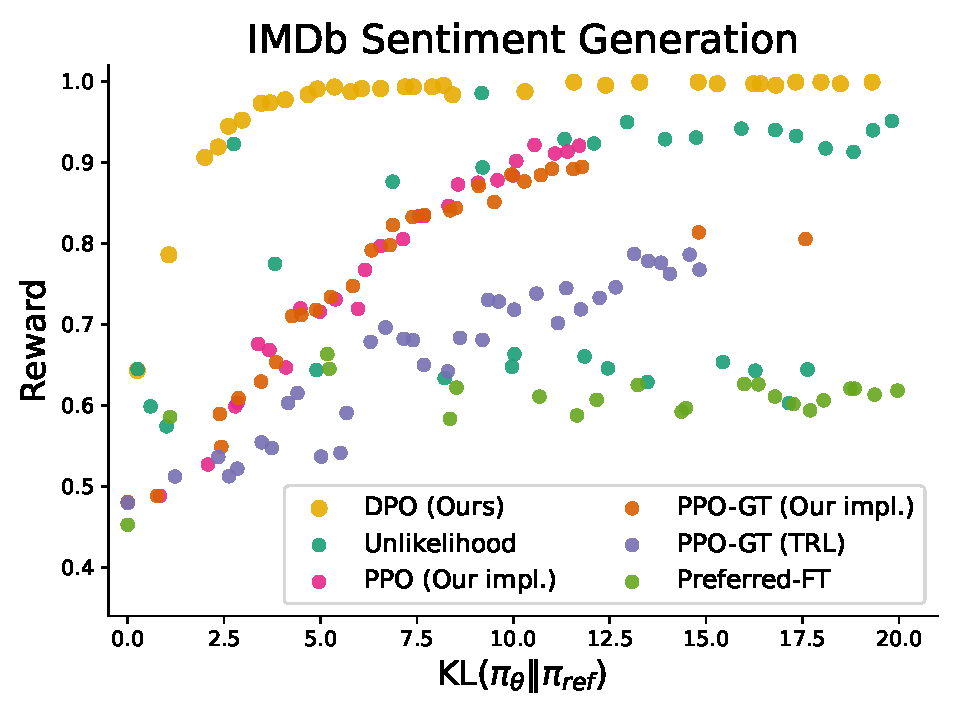
\includegraphics[width=\textwidth]{img/results/frontier.pdf}
		\end{column}
		\begin{column}{0.33\textwidth}
			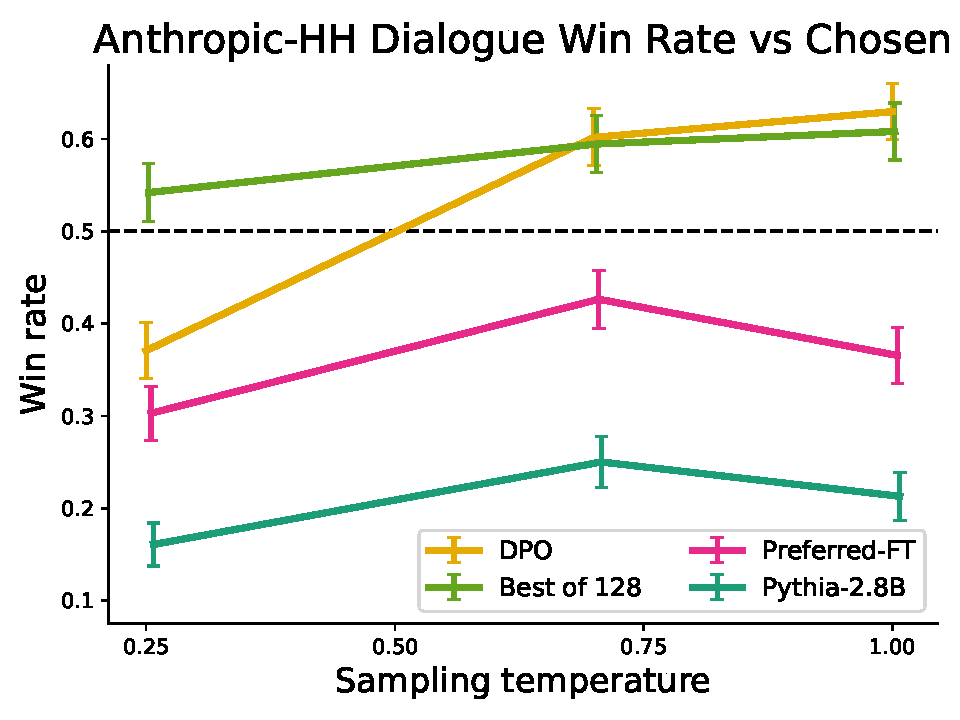
\includegraphics[width=\textwidth]{img/results/dialogue_winrate_vs_temp.pdf}
		\end{column}
		\begin{column}{0.34\textwidth}
			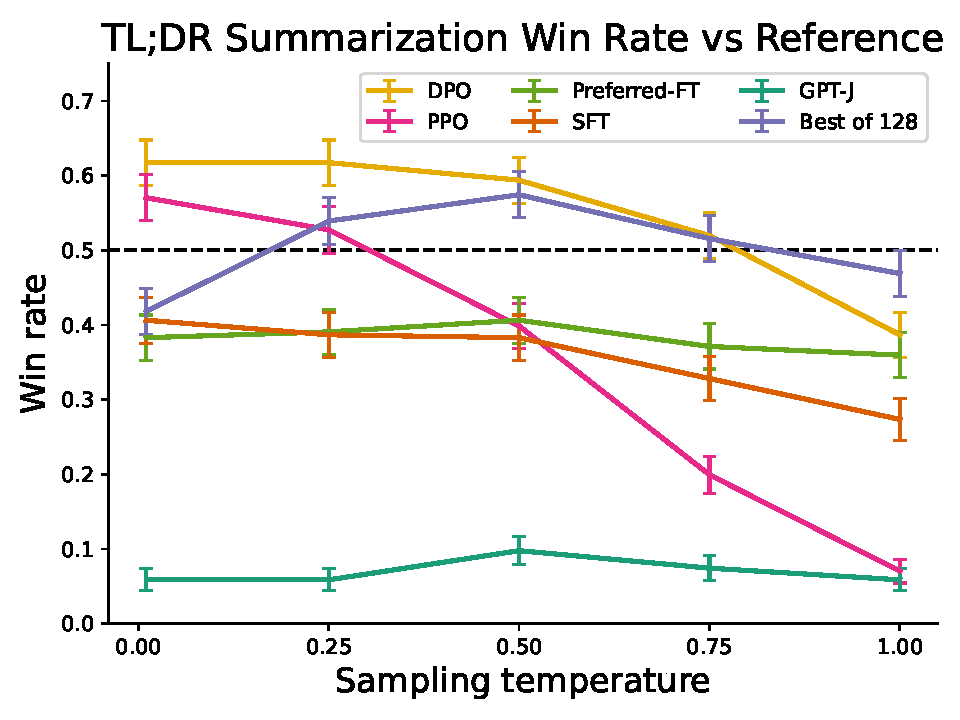
\includegraphics[width=\textwidth]{img/results/tldr_winrate_vs_temp.pdf}
		\end{column}
	\end{columns}
\end{frame}

\begin{frame}{Scalability}
	DPO was shown to \underline{work well at scale}, outperforming PPO \textit{without} tuning $\beta$. \pause It was also \underline{compared with human evaluators} for robustness:
	\begin{table}
		\small
		\begin{tabular}{lccc}
			\toprule
			& \textbf{DPO} & \textbf{SFT} & \textbf{PPO-1} \\
			\cmidrule(lr){2-4}
			N respondents & 272 & 122 & 199 \\
			\midrule
			GPT-4 (S) win \% & 47 & 27 & 13 \\
			GPT-4 (C) win \% & 54 & 32 & 12 \\
			Human win \% & 58 & 43 & 17 \\
			\midrule
			GPT-4 (S)-H agree & 70 & 77 & 86 \\
			GPT-4 (C)-H agree & 67 & 79 & 85 \\
			H-H agree & 65 & - & 87 \\
			\bottomrule
		\end{tabular}
	\end{table}
\end{frame}

\begin{frame}{Generalizability \& Future Work}
	To evaluate \textbf{generalizability}, DPO is also compared against PPO on out-of-distribution inference on CNN/DailyMail articles.
	\begin{table}
		\begin{tabular}{ccc}
			\toprule
			& \multicolumn{2}{c}{\textbf{Win rate vs. ground truth}} \\
			\cmidrule(lr){2-3}
			\textbf{Alg.} & Temp $0$ & Temp $0.25$ \\
			\midrule
			DPO & 0.36 & 0.31 \\
			PPO & 0.26 & 0.23 \\
			\bottomrule
		\end{tabular}
	\end{table}

	Here, DPO outperforms PPO \textit{despite} not using additional unlabelled prompts, that PPO requires.
	\pause \newline \\

	The authors note that more extensive study on the generalizability of DPO is necessary. \pause \newline \\

	Finally, DPO is also \textit{only} evaluated on 6B parameter models, and an exploration of it's performance at scale is also necessitated.
\end{frame}

\begin{frame}{Thank you!}
	\begin{center}
		Have an awesome rest of your day!
	\end{center}
	\begin{center}
		\textbf{Slides:} \url{https://cs.purdue.edu/homes/jsetpal/slides/dpo.pdf}
	\end{center}
\end{frame}

\end{document}
